\documentclass{standalone}
\usepackage{tikz}
\usetikzlibrary{calc, intersections}

\begin{document}
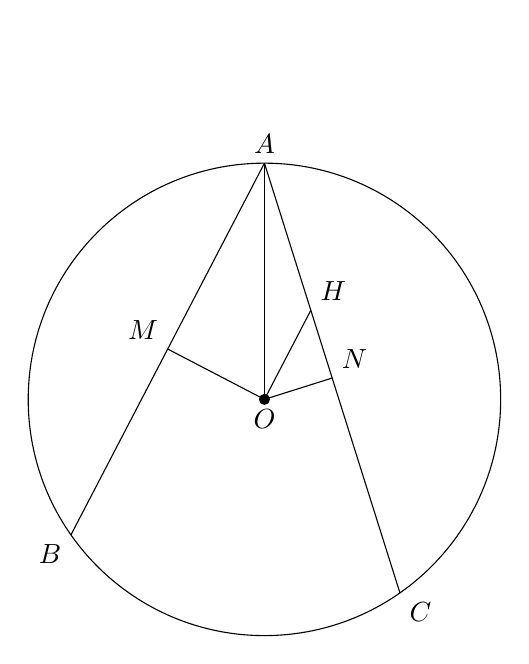
\begin{tikzpicture}
    % Define coordinates based on visual estimation of the original image
    \coordinate (O) at (0,0);
    \coordinate (A) at (90:3);
    % B is bottom-left, C is bottom-right. 
    % B is placed higher than C (angle 215 vs 305) to match the visual asymmetry 
    % where M is higher than N.
    \coordinate (B) at (215:3); 
    \coordinate (C) at (305:3);
    
    % M and N are midpoints of chords AB and AC respectively.
    % This corresponds to OM and ON being perpendicular to the chords,
    % which is consistent with the visual representation.
    \coordinate (M) at ($(A)!0.5!(B)$);
    \coordinate (N) at ($(A)!0.5!(C)$);
    
    % Draw the circle
    \draw (O) circle (3);
    
    % Draw chords AB and AC
    \draw (A) -- (B);
    \draw (A) -- (C);
    
    % Draw segments OA, OM, ON as in the original image
    \draw (O) -- (A);
    \draw (O) -- (M);
    \draw (O) -- (N);
    
    % New Instruction: Draw a line through O parallel to AB, intersecting AC at H.
    % The direction of AB is B - A. The parallel line through O has direction A - B (pointing up-right towards AC).
    \path[name path=lineOH] (O) -- ($(O) + (A) - (B)$);
    \path[name path=segAC] (A) -- (C);
    
    % Find intersection H
    \path[name intersections={of=lineOH and segAC, by=H}];
    
    % Draw segment OH
    \draw (O) -- (H);
    
    % Draw point O
    \fill (O) circle (2pt);
    
    % Labels
    \node[above] at (A) {$A$};
    \node[below left] at (B) {$B$};
    \node[below right] at (C) {$C$};
    \node[above left] at (M) {$M$};
    \node[above right] at (N) {$N$};
    \node[below] at (O) {$O$};
    \node[above right] at (H) {$H$};
\end{tikzpicture}
\end{document}
